\documentclass[12pt]{article}
\usepackage[utf8]{inputenc}

\usepackage[a4paper, margin=1in]{geometry}
\usepackage{newtxtext}
\usepackage{amsmath,amssymb,amsthm}
\usepackage{newtxmath} % must come after amsXXX

\usepackage{float} % to prevent figure floating

\usepackage{graphicx}

\usepackage{tabularx} % Include this in the preamble

%\usepackage{subfigure}

\usepackage{xcolor}
\usepackage{fancyhdr}
\usepackage{listings}
%\usepackage{ctex}
\usepackage{booktabs}

%%%%%%%%%%%% for pseudocode %%%%%%%
\usepackage{algorithm}
\usepackage{algpseudocode}
%%%%%%%%%%%%%%%%%%%%%%%%%%%%%%%%%%%

\usepackage{array}  % For wrapping text in columns
\usepackage{lipsum} % For placeholder text (optional)


\makeatletter
\renewcommand\paragraph{\@startsection{paragraph}{4}{\z@}%
% display heading, like subsubsection
                                     {-3.25ex\@plus -1ex \@minus -.2ex}%
                                     {1.5ex \@plus .2ex}%
                                     {\normalfont\normalsize\bfseries}}
 \setcounter{secnumdepth}{4}
\makeatother

\usepackage{amsmath,amsfonts,amssymb}
\usepackage{geometry}
\usepackage{graphicx}
\usepackage{caption}
\usepackage{fancyhdr}
\usepackage{titling}
\usepackage{lipsum}  % This package provides filler text, remove it in your actual document

\geometry{
 a4paper,
 total={170mm,257mm},
 left=20mm,
 top=20mm,
}

% Header and Footer settings
\pagestyle{fancy}
\fancyhf{}
\cfoot{\thepage}
\renewcommand{\headrulewidth}{0pt}
\renewcommand{\footrulewidth}{0pt}

\title{Falling Drop Simulation--Review}
\author{Haobo Zhao}
\date{\today}

\begin{document}

\maketitle

% \begin{abstract}
% This report presents a numerical simulation of the transient evolution of a falling drop in a two-fluid system, focusing on the deformation, breakup, and trajectory of the drop as it descends through a stationary fluid under the influence of gravity. The study utilizes the Volume of Fluid (VOF) method to track the interface between the immiscible fluids, capturing the complex interplay of forces such as buoyancy, inertia, viscosity, and surface tension. The governing equations are solved in a dimensionless form, characterized by the Reynolds and Bond numbers, to ensure generality and scalability to different physical systems. For computational efficiency, the governing parameters are chosen such that accurate results are obtained on a relatively coarse grid, while a grid refinement study confirms the validity of the solutions. The simulation provides insight into the dynamics of falling drops, such as shape deformation, terminal velocity, and the influence of varying nondimensional parameters, with potential applications in industrial processes, meteorology, and multiphase flow systems. The results are compared with prior literature to validate the model and identify avenues for future investigation.
% \end{abstract}

% \section{Introduction}
% The behavior of falling drops has garnered significant attention across various disciplines, including chemical engineering, environmental sciences, and industrial processes, due to its fundamental and practical implications in both natural and engineered systems. In nature, the dynamics of raindrops as they fall through the atmosphere affect precipitation patterns, while in industrial contexts, liquid droplets play a key role in processes such as spray drying, inkjet printing, and fuel atomization in combustion systems \cite{yarin2006drop, frohn2000dynamics}. Accurately predicting the motion, deformation, and breakup of a falling drop is crucial for optimizing performance in these systems.

% The dynamics of a falling drop are governed by the interplay of several physical forces, including gravity, inertia, surface tension, and viscous stresses. These forces collectively determine the drop's shape evolution, trajectory, and potential breakup as it moves through a quiescent fluid. 


% The study of these phenomena dates back to the pioneering work of Worthington \cite{worthington1876study}, who first captured the behavior of falling drops in detailed experimental studies. Since then, significant advancements have been made in both experimental and numerical methods for modeling drop dynamics. Modern approaches, such as those discussed in our well-known professor Prosperetti \cite{prosperetti2015life} and Tryggvason et al. \cite{tryggvason2011multiphase}, utilize high-fidelity numerical simulations to capture complex interactions between the fluid phases and the evolving interface.

% This study aims to numerically simulate the transient evolution of a falling drop in a two-fluid system using the Volume of Fluid (VOF) method. By selecting computationally convenient governing parameters, the simulation provides insights into the deformation and dynamics of the drop, with a focus on the effects of nondimensional numbers such as the Reynolds and Bond numbers. The results of this simulation are compared to existing literature to validate the model and explore the implications of varying these parameters on drop behavior.


\section{Introduction, Background}

\subsection{Introduction}





\subsection{Research Overview of Falling Drop Along time}

\begin{table}[htbp]
\scriptsize
\centering
\caption{Key Studies and Approaches on Drop Dynamics (Chronological Order)}
\renewcommand{\arraystretch}{1.2} % Adjust row height for better spacing
\begin{tabularx}{\textwidth}{|c|X|X|}
\hline
\textbf{Ref}                 & \textbf{Key Approach}                                                 & \textbf{Result/Contribution}                                                            \\ \hline
Stokes, 1851                 & Analytic solution for viscous drag on small spheres                    & Established Stokes' law, applicable to small falling droplets                           \\ \hline
Worthington, 1876            & First experimental capture of falling drop dynamics                    & Laid the experimental foundation for drop dynamics studies                              \\ \hline
Rayleigh, 1878               & Stability of liquid jets                                               & Foundation for instability phenomena in fluid dynamics                                  \\ \hline
Taylor, 1934                 & Study of emulsion formation in flow fields                             & Key insights into the relationship between surface tension and flow                     \\ \hline
Proudman \& Pearson, 1957    & Expansion at small Reynolds number                                     & Showed shape deformation and velocity relationship for falling droplets                 \\ \hline
Hirt \& Nichols, 1981        & Volume of Fluid (VOF) method for free boundary dynamics                & Developed a widely-used numerical method for multiphase flow simulations                \\ \hline
Brackbill et al., 1992       & Surface tension models in numerical methods                            & Introduced surface tension models into methods like VOF                                 \\ \hline
Peregrine et al., 1997       & Investigation of drop impact on liquid surfaces                        & Studied splashing phenomena during droplet impacts                                      \\ \hline
Eggers, 1997                 & Nonlinear dynamics and breakup of free-surface flows                   & Described the nonlinearity and singularities in droplet splitting                       \\ \hline
Han \& Tryggvason, 1999      & Axisymmetric drop breakup using CFD                                    & Studied drop breakup with parameters like Eo, Oh, Re, and We                            \\ \hline
Brenner et al., 1999         & Study of viscous liquid breakup                                        & Provided detailed analysis of droplet breakup mechanisms                                \\ \hline
Thoroddsen et al., 2008      & High-speed photography of droplet impacts                             & Captured droplet collision and fragmentation at extreme velocities                      \\ \hline
Popinet, 2009                & Accurate adaptive solver for interfacial flows                        & Developed Gerris, an open-source tool for high-precision simulation of droplet dynamics \\ \hline
Prosperetti, 2015            & Numerical simulations of fluid-fluid interactions with high accuracy   & Improved accuracy in the simulation of fluid-fluid interaction phenomena                \\ \hline
Fuster \& Popinet, 2018      & All-Mach method for bubble dynamics and surface tension simulations    & Provided simulations of complex two-phase flows with high performance computing         \\ \hline
\end{tabularx}
\end{table}


% \subsection{Overview of the Falling Drop Dynamics}

% The dynamics of a falling drop through a fluid medium, such as air or another liquid, involve complex physical processes that depend on various parameters, including fluid properties, drop size, velocity, and external forces such as gravity. Understanding these phenomena is critical in fields such as fluid mechanics, meteorology, inkjet printing, and spray technology. The evolution of a falling drop can be described in several stages:

% \subsubsection*{1. Initial Formation and Detachment}
% When a liquid drop detaches from a nozzle, surface tension forces dominate, pulling the drop into a spherical shape to minimize surface energy. The balance between surface tension, gravity, and inertia determines the size of the drop at detachment. Smaller drops are more spherical due to stronger surface tension forces relative to gravity \cite{worthington1876study}.

% \subsubsection*{2. Acceleration and Deformation}
% As the drop falls, it accelerates under gravity. If falling through air, the drag force exerted by the air increases as the drop's velocity increases. The shape of the drop may deform from a perfect sphere due to the balance between the drop’s inertia and the aerodynamic drag. The deformation depends on several dimensionless numbers:
% \begin{itemize}
%     \item \textbf{Reynolds number (Re)}: Characterizes the relative importance of inertial forces to viscous forces in the surrounding fluid. Higher Re typically results in more turbulent flow conditions and greater deformation.
%     \item \textbf{Bond number (Bo)}: Relates gravitational forces to surface tension. Larger Bo results in greater deformation, as gravity stretches the drop into an oblate shape \cite{tryggvason2011multiphase}.
% \end{itemize}

% \subsubsection*{3. Oscillation and Vibration}
% For sufficiently large drops, instabilities at the surface can cause oscillations and vibrations as the drop moves through the fluid. These oscillations arise from the interplay of inertia, surface tension, and drag. Surface tension restores the spherical shape, while inertia drives the oscillation. This behavior can be damped or amplified depending on drop size, speed, and the surrounding fluid \cite{hirt1981volume}.

% \subsubsection*{4. Terminal Velocity}
% As the drop continues to fall, drag force increases until it balances the gravitational force, leading to a constant velocity known as \textbf{terminal velocity}. The terminal velocity depends on the drop’s size, density, and the properties of the surrounding medium. For small water droplets falling in air, this terminal velocity is relatively low due to air resistance, but for larger drops, terminal velocity can be significantly higher \cite{prosperetti2015life}.

% \subsubsection*{5. Deformation and Breakup}
% At higher velocities or in more turbulent conditions, the drop experiences significant deformation. Two primary modes of deformation are observed:
% \begin{itemize}
%     \item \textbf{Oblate Deformation}: The drop flattens along its vertical axis due to aerodynamic drag.
%     \item \textbf{Internal Circulation}: Viscous forces induce internal fluid circulation, redistributing the drop's mass.
% \end{itemize}
% If the velocity or size exceeds a critical threshold, the drop undergoes \textbf{breakup}, fragmenting into smaller droplets. Common breakup modes include:
% \begin{itemize}
%     \item \textbf{Bag Breakup}: A thin film forms at the center and inflates outward, bursting into smaller droplets.
%     \item \textbf{Sheet or Strip Breakup}: Surface instabilities form elongated strips, fragmenting into droplets.
%     \item \textbf{Catastrophic Breakup}: For very large drops or high velocities, the drop explosively fragments into many small droplets \cite{brackbill1992continuum}.
% \end{itemize}

% \subsubsection*{6. Splashing Upon Impact}
% If the drop impacts a solid surface or another fluid, it may exhibit a range of behaviors:
% \begin{itemize}
%     \item \textbf{Spread}: The drop may spread into a thin sheet upon impact, especially on smooth surfaces.
%     \item \textbf{Rebound}: If the surface is hydrophobic or the velocity is low, the drop may retract and bounce off.
%     \item \textbf{Splashing}: At higher velocities, the drop splatters and ejects smaller satellite droplets. Splashing dynamics depend on surface roughness, impact speed, and fluid viscosity \cite{peregrine1997splashing}.
% \end{itemize}

% \subsubsection*{7. Influence of Physical Parameters}
% The behavior of falling drops is highly dependent on nondimensional numbers:
% \begin{itemize}
%     \item \textbf{Reynolds Number (Re)}: Higher Re numbers, often due to larger drops or faster velocities, lead to more turbulent flow conditions and increased drag.
%     \item \textbf{Weber Number (We)}: Represents the ratio of inertial forces to surface tension, where higher values lead to more severe deformations and breakup.
%     \item \textbf{Ohnesorge Number (Oh)}: Describes the influence of viscosity in the drop. High viscosity tends to suppress oscillations and breakup \cite{eggers1997nonlinear}.
% \end{itemize}
% Changes in temperature, viscosity, surface tension, or ambient pressure can significantly alter the drop's behavior. For example, lower surface tension or higher ambient pressures often result in greater deformations and more complex breakup dynamics.





% \section{Problem Formulation}
% The system involves a liquid drop falling through a stationary fluid under the influence of gravity. The problem is governed by the Navier-Stokes equations for incompressible flow:
% \begin{equation}
%     \rho \left( \frac{\partial \mathbf{u}}{\partial t} + \mathbf{u} \cdot \nabla \mathbf{u} \right) = -\nabla p + \mu \nabla^2 \mathbf{u} + \mathbf{F_g},
% \end{equation}
% where $\rho$ is the density, $\mathbf{u}$ is the velocity, $p$ is the pressure, $\mu$ is the dynamic viscosity, and $\mathbf{F_g}$ represents the gravitational force acting on the drop.

% The interface between the drop and the surrounding fluid is tracked using the Volume of Fluid (VOF) method, which is particularly suited for simulating two-fluid systems where interface deformation plays a key role.


\section{Solution Approach}
\subsection{Formulation}


\subsection{Numerical Approach}


\subsection{Parameters}







To construct the problem, we are using a finite domain to simulate the drop breakup, where the symbols and their description showing as follows:
\begin{table}[ht]
\scriptsize
\centering
\caption{Explanation of symbols and their corresponding values used in non-dimensional numbers}
\renewcommand{\arraystretch}{1.5} % Adjust row height
\begin{tabular}{|c|c|c|}
\hline
\textbf{Symbol} & \textbf{Description} & \textbf{Corresponding Value} \\ \hline
$t$     & Time & $1 \, \text{s}$ \\ \hline
$V$     & Initial relative velocity between the drop and surrounding fluid & $1 \, \text{m/s}$ \\ \hline
$D$     & Initial diameter of the drop & $1 \, \text{mm}$ \\ \hline
$\rho_0$ & Density of the liquid phase (e.g., the drop) & $1000 \, \text{kg/m}^3$ (water) \\ \hline
$\rho_1$ & Density of the surrounding fluid & $1.2 \, \text{kg/m}^3$ (air) \\ \hline
$\mu_0$  & Viscosity of the liquid phase (drop) & $0.001 \, \text{Pa·s}$ (water) \\ \hline
$\mu_1$  & Viscosity of the surrounding fluid & $1.8 \times 10^{-5} \, \text{Pa·s}$ (air) \\ \hline
$\sigma$ & Surface tension at the interface between the liquid and the surrounding fluid & $0.072 \, \text{N/m}$ (water-air interface) \\ \hline
$a_z$ & Acceleration (e.g., gravitational acceleration) & $9.81 \, \text{m/s}^2$ \\ \hline
$\Delta \rho$ & Density difference between the drop and surrounding fluid & $998.8 \, \text{kg/m}^3$ \\ \hline
$g$ & Gravitational acceleration & $9.81 \, \text{m/s}^2$ \\ \hline
\end{tabular}
\label{tab:SymbolExplanations}
\end{table}

\subsection{Nondimensional Numbers}
% We need non-dimensional time, which could lead more accurate comparison with the literature.
% \begin{equation}
%     t^* = \frac{tV}{D}
% \end{equation}

% Where, V is initial relative velocity, and D is the drop's initial diameter.

% \begin{equation}
%     We = \frac{\rho_0 V^2 D}{\sigma}
% \end{equation}

% \begin{equation}
%     Re = \frac{\rho_9 V D}{\mu_0}
% \end{equation}



We are using the non-dimensional numbers showing as follows:


\begin{table}[H]
\scriptsize
\centering
\caption{Non-dimensional numbers in drop dynamics and their physical significance}
\renewcommand{\arraystretch}{1.2} % Adjust row height for better spacing
\begin{tabularx}{\textwidth}{|c|c|X|c|X|}
\hline
\textbf{Symbol} & \textbf{Name} & \textbf{Definition and Physical significance} & \textbf{Typical Value} & \textbf{Example in Real Systems} \\ \hline
$t^* = \frac{t}{\sqrt{D/a_z}}$ & Non-dimensional time & Time scaled by drop diameter and acceleration & $0.1$ to $10$ & Rain droplet falling under gravity \\ \hline
$Eo = \frac{\Delta \rho g D^2}{\sigma}$ & Eötvös number & Ratio of gravitational forces to surface tension forces & $10^{-2}$ to $10^2$ & Large rain droplet or industrial liquid flows \\ \hline
$Oh_d = \frac{\mu_d}{\sqrt{\rho_d D \sigma}}$ & Ohnesorge number (drop) & Ratio of viscous forces to inertial and surface tension forces & $0.01$ to $0.1$ & Small liquid droplets like water in air \\ \hline
$Oh_o = \frac{\mu_o}{\sqrt{\rho_o D \sigma}}$ & Ohnesorge number (surrounding fluid) & Ratio of viscous forces to inertial and surface tension forces & $0.1$ to $1$ & Liquid droplets in highly viscous fluids \\ \hline
$\rho^* = \frac{\rho_d}{\rho_o}$ & Density ratio & Ratio of the density of the drop to the surrounding fluid & $1.1$ to $10^3$ & Water droplets in air or oil-water systems \\ \hline
$\mu^* = \frac{\mu_d}{\mu_o}$ & Viscosity ratio & Ratio of the viscosity of the drop to the surrounding fluid & $10^{-3}$ to $1$ & Liquid droplets in oil or water \\ \hline
\end{tabularx}
\label{tab:NonDimensionalNumbersSignificance}
\end{table}


\subsection{Non-Dimensional number's control using $a_z$ and $\mu_D$}


As the major non-dimensional numbers are Ohnesorge number and Eotvos number, we use our basic parameters to control them:



\begin{align}
    a_z  &= \frac{\sigma Eo}{\Delta \rho D^2} = \frac{100Eo}{12} 
    \hspace{0.2\textwidth} 
    & \mu_D &= Oh_d \sqrt{\rho_d D \sigma} = \sqrt{6000} \, Oh_d
\end{align}

\begin{minipage}[t]{0.45\textwidth}
    \centering
    \captionof{table}{Parameter Values 1}
    \begin{tabular}{|c|c|c|c|c|c|}
        \hline
        $\rho_o$ & $\rho_d$ & $\Delta \rho$ & $D$ & $\sigma$ & $a_z$  \\ \hline
        1 & 10 & 9 & 2 & 300 &  $\frac{100 Eo}{\sigma}$ \\ \hline
    \end{tabular}
\end{minipage}
\hfill
\begin{minipage}[t]{0.45\textwidth}
    \centering
    \captionof{table}{Parameter Values 2}
    \begin{tabular}{|c|c|c|c|c|c|}
        \hline
        $\rho_o$ & $\rho_d$ & $\Delta \rho$ & $D$ & $\sigma$ & $a_z$  \\ \hline
        1 & 10 & 9 & 2 & 300 &  $\frac{100 Eo}{\sigma}$ \\ \hline
    \end{tabular}
\end{minipage}





\section{Simulation Setup}
\subsection{Domain and Boundary Condition}
The Domain is set up as follows:
\begin{figure}[H]
    \centering
    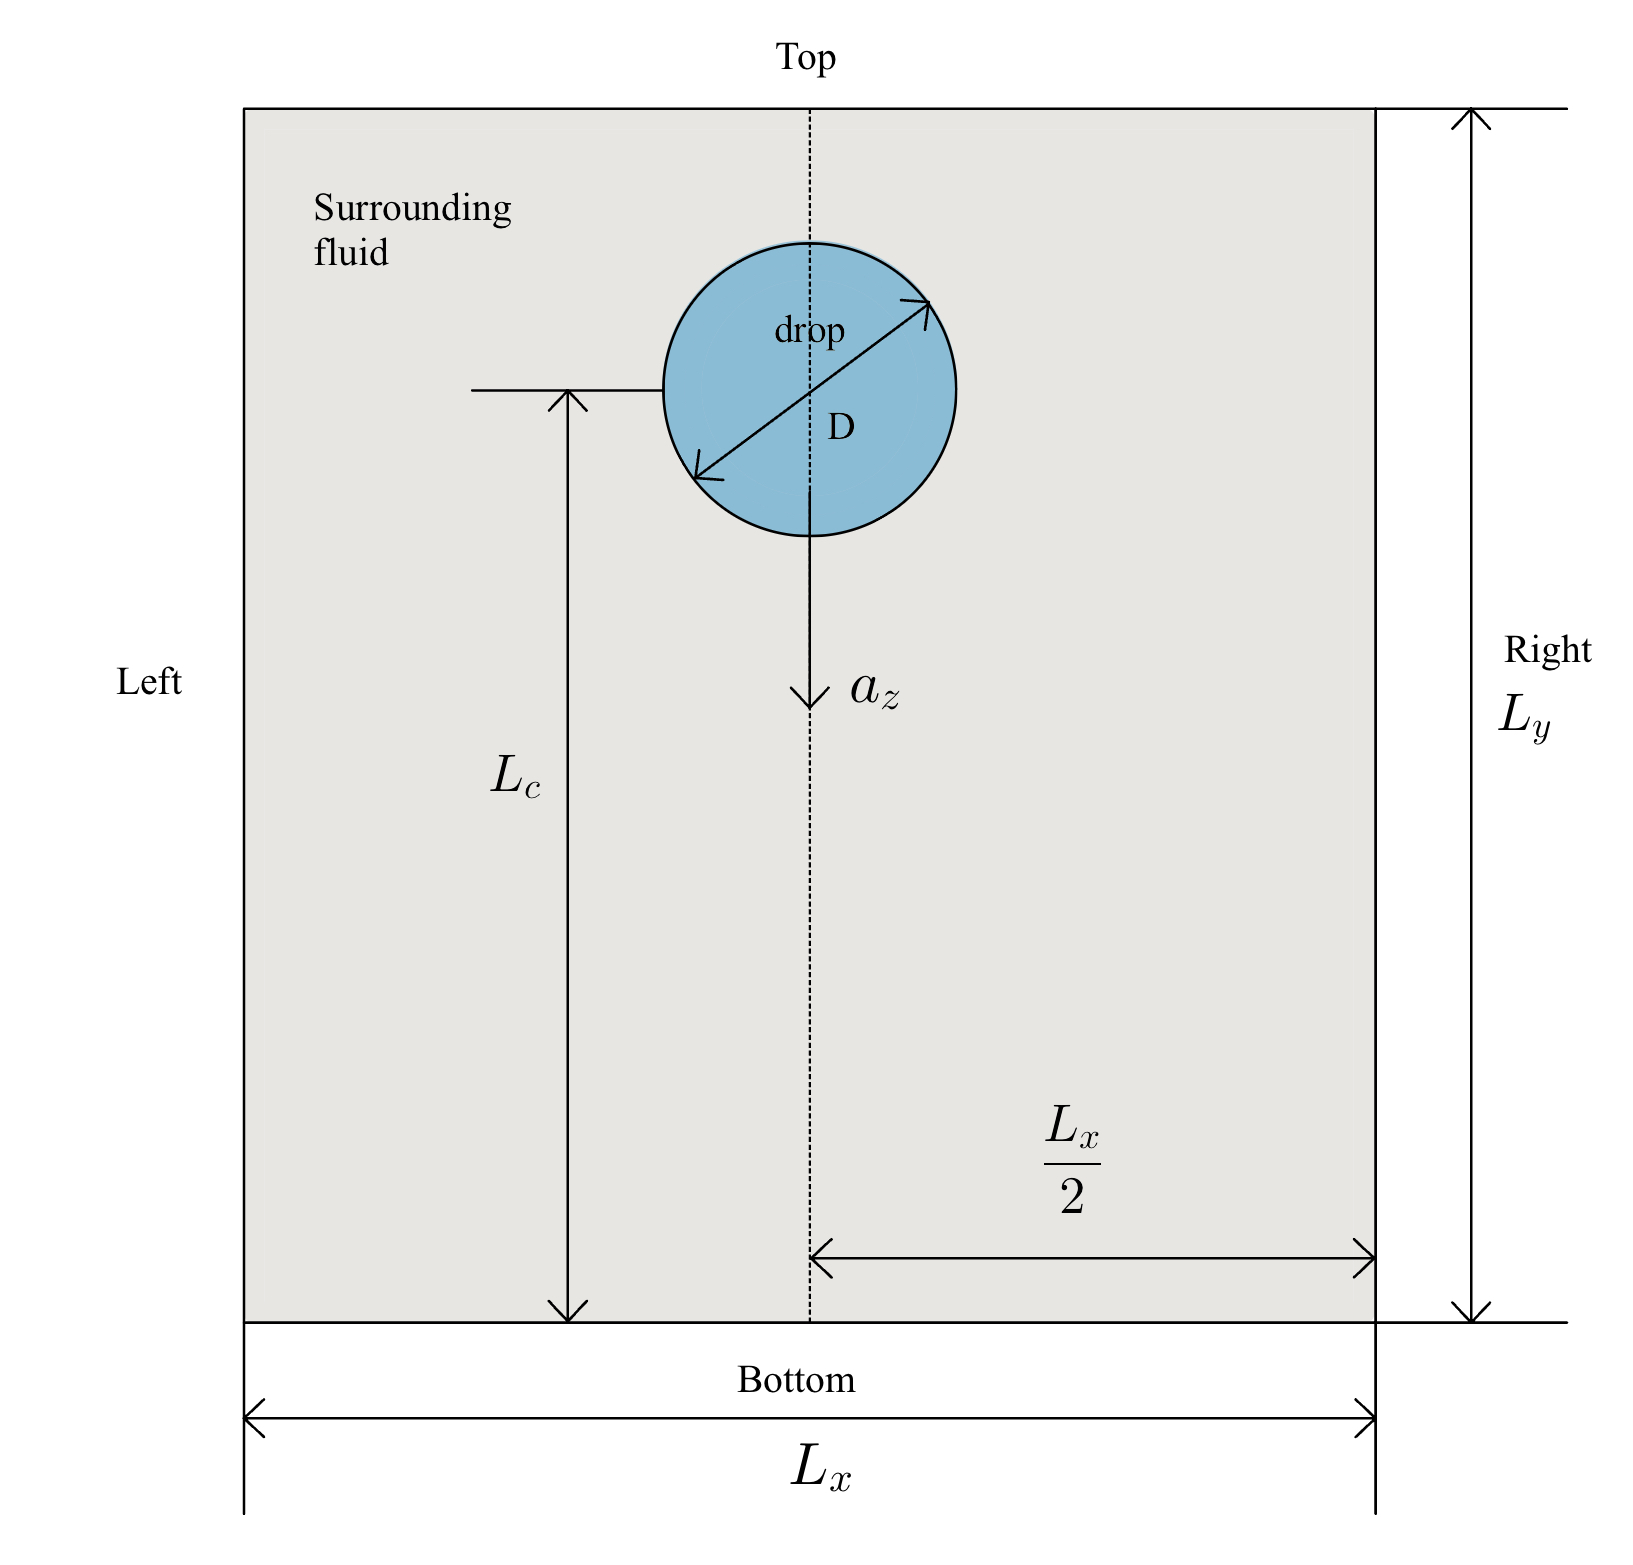
\includegraphics[width=0.6\textwidth]{Latex/figures/Domain.jpg}
    % \caption{Drop deformation as a function of the Reynolds number.}
    \label{deformation}
\end{figure}



\begin{table}[ht]
\scriptsize
\centering
% \caption{Explanation of symbols and their corresponding values used in non-dimensional numbers}
\renewcommand{\arraystretch}{1.5} % Adjust row height
\begin{tabular}{|c|c|c|c|c|c|c|c|}
\hline
\multicolumn{4}{|c|}{\textbf{Length}} & \multicolumn{4}{c|}{\textbf{Boundary condition}} \\
\hline
$L_x$ & $L_y$ & $L_c$ & $D$   & Top & Bottom & Left & Right \\
\hline
$10D$ & $30D$ & $0.9L_y$ & $D$   & Symm & Symm & Symm & Symm \\
\hline
\end{tabular}
\end{table}















\subsection{Result}
\subsubsection{Compare to Perivous Result}



\subsubsection{Grid Independence Study}

\subsubsection{Key Parameters Along time}

\begin{figure}[H]
    \centering
    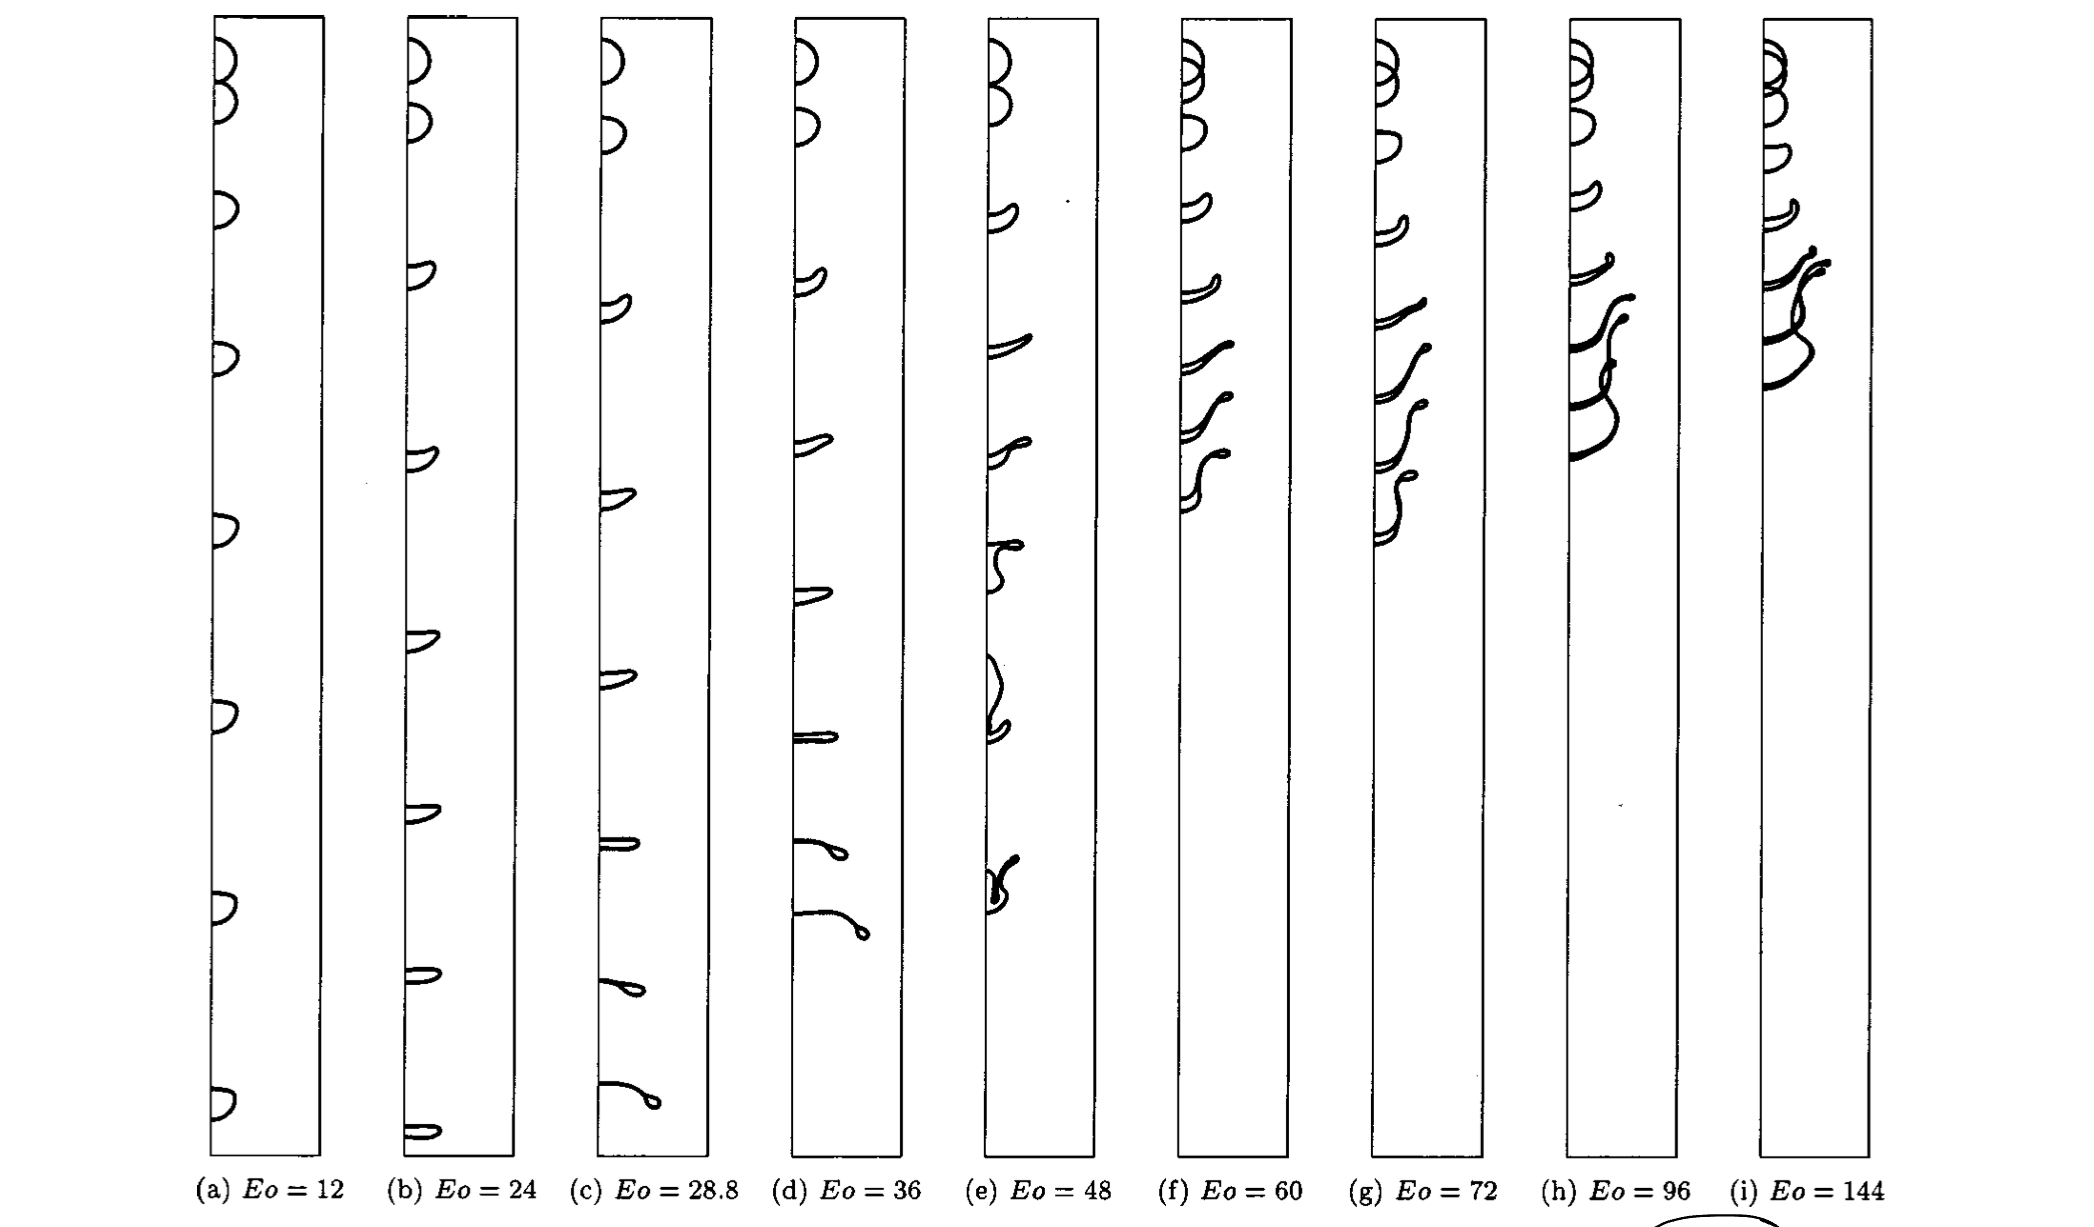
\includegraphics[width=\textwidth]{Latex/figures/Trygg_allEo.jpg}
    \caption{Drop deformation as a function of the Reynolds number.}
    \label{deformation}
\end{figure}


\begin{tabular}{|>{\centering\arraybackslash}m{1cm} |>{\centering\arraybackslash}m{1cm} |>{\centering\arraybackslash}m{1cm} |>{\centering\arraybackslash}m{1cm} |>{\centering\arraybackslash}m{1cm} |>{\centering\arraybackslash}m{1cm} |>{\centering\arraybackslash}m{1cm} |>{\centering\arraybackslash}m{1cm} |>{\centering\arraybackslash}m{1cm} |>{\centering\arraybackslash}m{1cm}|}
\hline
\textbf{Eo} & 12 & 24 & 28.8 & 36 & 48 & 60 & 72 & 96 & 144 \\
\hline
\textbf{Last time $t^*$} & 11.19 & 15.82 & 14.85 & 13.83 & 11.19 & 7.15 & 7.83 & 6.78 & 5.54 \\
\hline
\end{tabular}





\end{document}
















For this simulation, we chose $Re = 100$ and $Bo = 10$, which provide a computationally convenient yet physically relevant scenario.

\section{Numerical Method}
The simulation was carried out using the Volume of Fluid (VOF) method implemented in COMSOL/Matlab. A coarse grid was used to expedite computations, with grid refinement studies ensuring the accuracy of the results.

\section{Results}
The following figures show the transient evolution of the drop as it falls through the fluid. The shape of the drop changes as a function of time due to gravity and surface tension.

\begin{figure}[h!]
    \centering
    \includegraphics[width=0.8\textwidth]{drop_fall_frame1.png}
    \caption{Drop shape at $t = 0.1s$.}
\end{figure}

\begin{figure}[h!]
    \centering
    \includegraphics[width=0.8\textwidth]{drop_fall_frame2.png}
    \caption{Drop shape at $t = 0.5s$.}
\end{figure}

\begin{figure}[h!]
    \centering
    \includegraphics[width=0.8\textwidth]{drop_fall_frame3.png}
    \caption{Drop shape at $t = 1.0s$.}
\end{figure}

In addition, the evolution of the drop's centroid location over time is shown in Figure \ref{centroid}. The falling velocity and the influence of surface tension are clearly visible.

\begin{figure}[h!]
    \centering
    \includegraphics[width=0.8\textwidth]{centroid_vs_time.png}
    \caption{Centroid location of the drop as a function of time.}
    \label{centroid}
\end{figure}

\section{Grid Refinement Study}
To ensure accuracy, a grid refinement study was conducted by comparing the results on coarse and fine grids. Figure \ref{refinement} shows that the solution converges as the grid is refined, confirming the accuracy of the coarse grid results used for computational efficiency.

\begin{figure}[h!]
    \centering
    \includegraphics[width=0.8\textwidth]{grid_refinement.png}
    \caption{Grid refinement study showing convergence of the solution.}
    \label{refinement}
\end{figure}

\section{Effect of Varying Nondimensional Numbers}
Additional simulations were performed to study the effect of varying the Reynolds and Bond numbers. For example, increasing the Reynolds number from 100 to 200 resulted in more pronounced deformation of the falling drop, as illustrated in Figure \ref{deformation}.

\begin{figure}[h!]
    \centering
    \includegraphics[width=0.8\textwidth]{deformation_vs_re.png}
    \caption{Drop deformation as a function of the Reynolds number.}
    \label{deformation}
\end{figure}

\section{Discussion}
The results show that the drop falls with increasing deformation as the Reynolds number increases, consistent with earlier studies. The use of a coarse grid allowed for fast simulations, and grid refinement confirmed the accuracy of the results. Further work could explore the impact of surface tension and drop-wall interactions in more detail.

\section{Conclusion}
This simulation demonstrated the transient evolution of a falling drop in a two-fluid system. By selecting computationally convenient parameters, accurate results were obtained on a coarse grid. Future work could explore more complex drop behaviors or interactions with solid boundaries.

\bibliographystyle{plain}
\bibliography{references}

\end{document}
